\documentclass[aspectratio=169]{beamer}


\usetheme{metropolis} 
\usepackage[style=verbose-note, url=true]{biblatex}
\usepackage{graphicx,microtype,geometry,listings}
\addbibresource{main.bib}

% Presentation information
\title{OTel Without Reservations}
\author{Ethan Kent}
\date{\today}

\begin{document}

\begin{frame}
  \titlepage
\end{frame}

\begin{frame}{Overview}
  \tableofcontents
\end{frame}

\section{Introduction}
\begin{frame}{What is OpenTelemetry?}

  According to the OpenTelemetry people,\footnote{OpenTelemetry is a project of
    The Cloud Native Computing Foundation and is a merger of the OpenTracing and
    OpenCensus projects.}

  \vspace{1em}

  \begin{quote}
    OpenTelemetry is a collection of tools, APIs, and SDKs. Use it to
    instrument, generate, collect, and export telemetry data (metrics, logs, and
    traces) to help you analyze your software's performance and
    behavior.\footcite{otel-site}
  \end{quote}
\end{frame}

\begin{frame}{Why do I care?}
  \begin{quote}

    A \emph{distributed trace}, more commonly known as a \emph{trace}, records
    the paths taken by requests (made by an application or end-user) as they
    propagate through multi-service architectures, like microservice and
    serverless applications.

    \vspace{0.618em}

    Without tracing, it is challenging to pinpoint the cause of performance
    problems in a distributed system.

    \vspace{0.618em}

    It improves the visibility of our application or system's health and lets us
    debug behavior that is difficult to reproduce locally. Tracing is essential
    for distributed systems, which commonly have nondeterministic problems or are
    too complicated to reproduce locally.\footcite{otel-dist-trace}

  \end{quote}
\end{frame}

\begin{frame}{Why do I care? (cont'd)}
  \begin{center}
    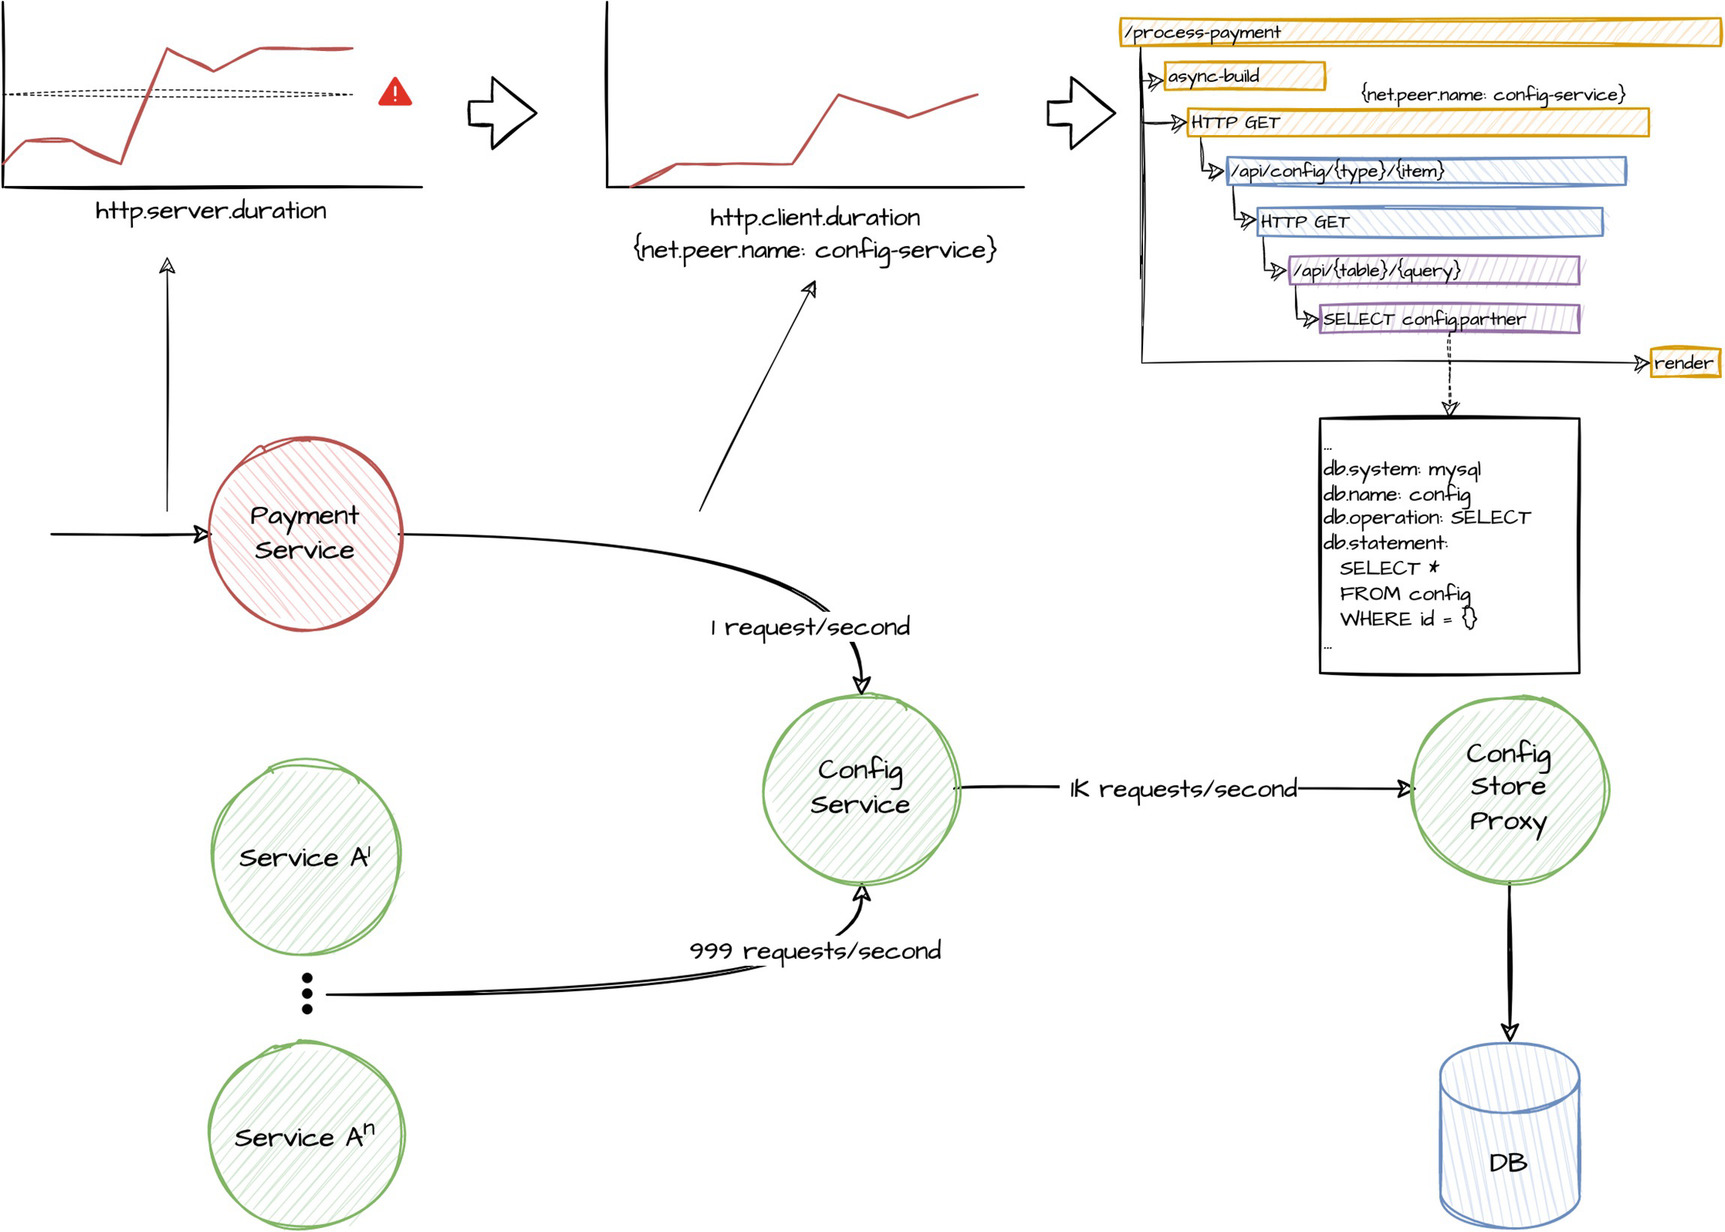
\includegraphics[width=0.9\textwidth, height=0.9\textheight, keepaspectratio]{distributed-tracing.jpg}
  \end{center}
\end{frame}

\begin{frame}{Why do I care? (cont'd)}
  \begin{description}
    \item[Observability] OpenTelemetry (OTel) offers comprehensive observability
      across your systems. OTel provides a clear picture of what's happening
      within your services by bringing together traces, metrics, and logs.
    \item[Reduced Complexity] OTel unifies multiple observability signals into a
      coherent framework. A single framework simplifies instrumentation and
      eliminates the need to learn and manage various systems.
    \item[Standards-Based] OTel is open-source and vendor-neutral, providing
      standardized APIs and instrumentation that integrates with any backend.
    \item[Extensibility] OTel's modular design allows you to use what you need,
      and its SDKs let you build custom integrations as required.
    \item[Cost and Resource Efficient] OTel can reduce the overhead and costs of
      running multiple observability tools.
  \end{description}
\end{frame}

\begin{frame}{Why do I care? (cont'd)}
  \begin{description}
    \item[Support for Modern Architectures] OTel provides first-class support
      for Kubernetes, serverless functions, and service meshes.
    \item[Enhanced Debugging] With better visibility, engineers can identify,
      understand, and resolve issues faster.
    \item[Performance Monitoring] OTel helps you monitor system performance and
      user behavior in real-time, helping you make data-driven decisions to
      improve your services' performance and user experience.
    \item[Future-Proof] OTel's wide adoption and large community likely mean
      that as new standards and best practices emerge, OTel will evolve with them.
  \end{description}
\end{frame}

\section{Signals}

\begin{frame}{Signals}
  ``In OpenTelemetry, a signal refers to a category of telemetry.''\footcite{otel-signals}

  \vspace{1em}

  The four kinds of signals currently supported are

  \begin{itemize}
    \item Traces,
    \item Metrics,
    \item Logs, and
    \item Baggage.\footcite{otel-signals}
  \end{itemize}
\end{frame}

\begin{frame}{Traces}
  \emph{Spans} are the bread and butter of distributed tracing. A \emph{Trace}
  has many \emph{Spans}.

  \vspace{1em}

  \begin{quote}
    Traces give us the big picture of what happens when a request is made to an
    application. Whether your application is a monolith with a single database
    or a sophisticated mesh of services, traces are essential to understanding
    the full ``path'' a request takes in your application.\footcite{otel-traces}
  \end{quote}
\end{frame}

\begin{frame}{Metrics}

  \begin{quote}

    A metric is a measurement about a service, captured at runtime. Logically,
    the moment of capturing one of these measurements is known as a metric event
    which consists not only of the measurement itself, but the time that it was
    captured and associated metadata.\footcite{otel-metrics}

  \end{quote}
\end{frame}

\begin{frame}{Metrics (cont'd)}

  Use metrics when you want metrics.

  \vspace{1em}

  \begin{quote}

    Some telemetry backends allow to execute ad hoc queries on spans, [and it]
    is also possible to derive metrics from spans in OpenTelemetry Collectors.
      {\Large This often results in an overuse of spans as a substitute for
        metrics when teams start to adopt tracing.} Trace sampling can affect any
    interpretations extracted directly from spans,~.~.~. [and] the high volumes
    of data and cardinality processed by trace pipelines in high-throughput
    systems normally result in signals that are less stable than metrics
    originating directly from a service~.~.~.~.\footcite[ch.~6, emphasis
      added]{practical-otel}

  \end{quote}
\end{frame}

\begin{frame}{Logs}
  \begin{quote}

    In OpenTelemetry, any data that is not part of a distributed trace or a
    metric is a log. For example, events are a specific type of log. Logs often
    contain detailed debugging/diagnostic info, such as inputs to an operation,
    the result of the operation, and any supporting metadata for that
    operation.\footcite{otel-logs}

  \end{quote}
\end{frame}

\begin{frame}{Logs: not well-supported yet}
  \begin{center}
    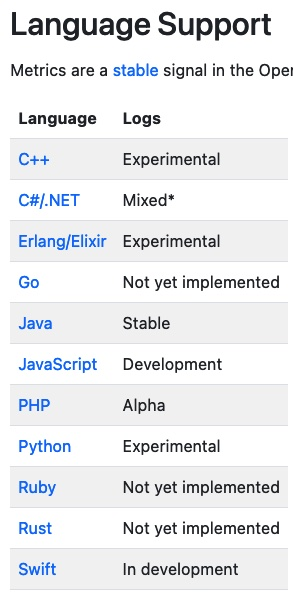
\includegraphics[height=0.8\textheight]{logs-support.jpg}
  \end{center}
\end{frame}

\begin{frame}{Baggage}
  ``In OpenTelemetry, Baggage is contextual information that's passed between
  spans. It's a key-value store that resides alongside span context in a trace,
  making values available to any span created within that trace.''\footcite{otel-baggage}

  It's in the HTTP headers, so don't store sensitive data.

  ``Common use cases include~.~.~. Account Identification, User Ids, Product
  Ids, and origin IPs.~.~.~.  Passing these down your stack allows you to then
  add them to your Spans in downstream services to make it easier to filter when
  you're searching in your Observability back-end.''\footcite{otel-baggage}
\end{frame}

\section{Context and Context Propagation}

\begin{frame}{How does this distributed stuff work?}

  Distributed tracing is hard because it's tricky to reconstruct cause and
  effect. In distributed systems, many separate services---some internal and
  some external---may collaborate to produce a final result. The secret sauce
  for OpenTelemetry can be split into three pieces:

  \begin{enumerate}
    \item A trace ID, additional correlation IDs, and other metadata,
          collectively called ``Context.''
    \item Standards governing how Context is transmitted within and among
          services, called ``Context Propagation.''
    \item An ecosystem comprising open standards, libraries, SDKs, vendors, etc.
  \end{enumerate}

  \vspace{1em}

  In short, OpenTelemetry is a well-thought-out system for assigning IDs in a
  tree-like structure, passing them across service boundaries, and allowing
  Humpty-Dumpty to be put back together again.

\end{frame}

\begin{frame}{Context}
  \begin{quote}

    A \texttt{Context} is a propagation mechanism which [sic] carries
    execution-scoped values across API boundaries and between logically associated
    execution units.  Cross-cutting concerns access their data in-process using
    the same shared \texttt{Context} object.\footcite{otel-context}

  \end{quote}

  \vspace{1em}

  \begin{quote}

    \begin{description}
      \item[Execution Unit] An umbrella term for the smallest unit of sequential
        code execution, used in different concepts of multitasking. Examples are
        threads, coroutines or fibers.\footcite{otel-defs}
    \end{description}

  \end{quote}

\end{frame}


\section{Auto SDK}
\section{Manual}

\section{Collectors and Exporters}

\section{Backends}
% \section{Instrumentation}
% \begin{frame}{Adding Instrumentation}
%   % Content goes here
% \end{frame}

% \section{Collectors and Exporters}
% \begin{frame}{Data Collection and Export}
%   % Content goes here
% \end{frame}

% \section{Visualizing and Analyzing Data}
% \begin{frame}{Tools and Dashboards}
%   % Content goes here
% \end{frame}

% \section{Use Cases}
% \begin{frame}{Real-World Use Cases}
%   % Content goes here
% \end{frame}

% \section{Conclusion}
% \begin{frame}{Summary and Next Steps}
%   % Content goes here
% \end{frame}
\end{document}
